% ------------------------------------------------------------------------
% bjourdoc.tex for birkjour.cls*******************************************
% ------------------------------------------------------------------------
%%%%%%%%%%%%%%%%%%%%%%%%%%%%%%%%%%%%%%%%%%%%%%%%%%%%%%%%%%%%%%%%%%%%%%%%%%

\documentclass{birkjour}

\usepackage[utf8]{inputenc}

\usepackage{amsmath}
\usepackage{xspace}
\usepackage{url}
\usepackage{rotating}
\usepackage{commands}
\usepackage{comment}
\usepackage{booktabs}
\usepackage{modallogics}
\usepackage{xcolor}
\usepackage[backend=biber,sorting=ydnt,maxnames=999,maxcitenames=999,maxbibnames=999,natbib]{biblatex}
\addbibresource[label=bibs]{Bibliography.bib}


\newcommand{\AOE}{$\mathcal{AOE}$}
\newcommand{\AOEH}{$\mathcal{AOE}'$}
\newcommand{\AOEHH}{$\mathcal{AOE}'_0$}
\newcommand{\AOEHHH}{$\mathcal{AOE}''$}



%
%
% THEOREM Environments (Examples)-----------------------------------------
%
 \newtheorem{thm}{Theorem}[section]
 \newtheorem{cor}[thm]{Corollary}
 \newtheorem{lem}[thm]{Lemma}
 \newtheorem{prop}[thm]{Proposition}
 \theoremstyle{definition}
 \newtheorem{defn}[thm]{Definition}
 \theoremstyle{remark}
 \newtheorem{rem}[thm]{Remark}
 \newtheorem*{ex}{Example}
 \numberwithin{equation}{section}

\def\HOML{\entity{HOML}\xspace}
\def\HOL{\entity{HOL}\xspace}


\begin{document}

%-------------------------------------------------------------------------
% editorial commands: to be inserted by the editorial office
%
%\firstpage{1} \volume{228} \Copyrightyear{2004} \DOI{003-0001}
%
%
%\seriesextra{Just an add-on}
%\seriesextraline{This is the Concrete Title of this Book\br H.E. R and S.T.C. W, Eds.}
%
% for journals:
%
%\firstpage{1}
%\issuenumber{1}
%\Volumeandyear{1 (2004)}
%\Copyrightyear{2004}
%\DOI{003-xxxx-y}
%\Signet
%\commby{inhouse}
%\submitted{March 14, 2003}
%\received{March 16, 2000}
%\revised{June 1, 2000}
%\accepted{July 22, 2000}
%
%
%
%---------------------------------------------------------------------------
%Insert here the title, affiliations and abstract:
%


\title[The Anderson-Hájek Ontological Controversy]
{Computer-Assisted Analysis of the \\
Anderson-Hájek Ontological Controversy}



%----------AUTHOR 1
\author[Benzm\"uller]{C. Benzm\"uller}

\address{%
Dep.~of Mathematics and Computer Science, Freie Universit\"at Berlin, Germany
}
\email{c.benzmueller@fu-berlin.com}

\thanks{This work was supported by German National Research Foundation (DFG) under
 grants BE 2501/9-1 and BE 2501/11-1.}


%----------Author 2
\author[Weber]{L. Weber}
\address{
Dep.~of Mathematics and Computer Science, Freie Universit\"at Berlin, Germany
}
\email{leon.weber@fu-berlin.de}


%----------Author 3
\author[Woltzenlogel-Paleo]{B. Woltzenlogel Paleo}
\address{
Room HA0402, Favoritenstra{\ss}e 9, 1040 Wien, Austria
}
\email{bruno.wp@gmail.com}




%----------classification, keywords, date
% \subjclass{
% % Prim. 03A02;  % Philosophical aspects of logic and foundations
% % Sec. 68T02 % Artificial Intelligence
% }

%\keywords{Ontological Argument, Modal Collapse}

\date{\today}
%----------additions
\dedicatory{ }
%%% ----------------------------------------------------------------------

% \begin{abstract}
% \end{abstract}

%%% ----------------------------------------------------------------------
\maketitle
%%% ----------------------------------------------------------------------
%\tableofcontents


\section{Introduction}
We present an exemplary study in \emph{Computational Metaphysics},
which is an emerging, interdisciplinary field aiming at the rigorous
formalisation and deep logical assessment of rational, philosophical
arguments on the computer.  The particular focus here is on the
ontological argument for the existence of God.  While related work
\citep{oppenheimer11,rushby13} has concentrated on Anselm's simpler original
version of the ontological argument and formalized it in classical
predicate logic, we here focus on modern variants of it requiring
higher-order modal logic. More precisely, the variants studied here are
all emendations of Kurt Gödel's seminal contribution
\citep{GoedelNotes}, respectively, Dana Scott's variant of it
\cite{ScottNotes} (cf. Fig.~\ref{fig:Goedel}). 

In preceding experiments \citep{C55,C40,J30}, we have already
demonstrated that the technology we employ is well suited for the
task. In fact, computers may even contribute philosophically relevant
new knowledge. For example, the theorem prover Leo-II \cite{Leo-II}
detected an inconsistency in Gödel's original script
\citep{GoedelNotes} of the argument, which was undetected by
philosophers before.  This inconsistency obviously renders Gödel's
original version of the argument as pointless.  However, as our
preceding experiments also confirmed, Scott's variant
\citep{ScottNotes} from Fig.~\ref{fig:Goedel} is immune to this
issue.\footnote{Gödel avoids the first conjunct $\varphi(x)$ in the
  definition of \emph{essence (D2)}, which Scott added for cosmetic
  reason. However, as Leo-II detected, one can prove from Gödel's
  definition that the empty property becomes an essence of every
  individual, which, together with theorem T1, axiom A5 and the
  defintion of \emph{necessary existence (D3)} causes the
  inconsistency. For more details see \citet{C55}.} Hence, in the
remainder of this article the term \emph{Gödel's ontological argument}
actually refers to Scott's variant of it, whose soundness has been
formally 
verified with our technology (for logics entailing higher-order modal
logic KB with constant domain or varying domain semantics). We here
assume some familiarity with these related experiments and papers.

\begin{figure}[t]
\noindent \framebox[\columnwidth][r]{
\begin{minipage}{.94\columnwidth}\small
\begin{itemize}
\item[A1] Either a property or its negation is positive, but not
  both:
  $$\hol{\allq \varphi [P(\neg \varphi) \biimp \neg P(\varphi)]}$$
\item[A2] A property necessarily implied by a
  positive property is positive:
  $$\hol{\allq \varphi \allq \psi [(P(\varphi) \wedge \nec \allq x [\varphi(x)
  \imp \psi(x)]) \imp P(\psi)]}$$
\item[T1] Positive properties are possibly exemplified:
  $$\hol{\allq \varphi [P(\varphi) \imp \pos \exq x \varphi(x)]}$$
\item[D1] A \emph{God-like} being possesses all positive properties:
  $$\hol{G(x) \equiv \forall \varphi [P(\varphi) \imp \varphi(x)]}$$
\item[A3]  The property of being God-like is positive:
  $$\hol{P(G)}$$
\item[C\phantom{1}] Possibly, a God-like being exists: $$\hol{\pos \exq x G(x)}$$
\item[A4]  Positive properties are necessarily positive:
  $$\hol{\allq \varphi [P(\varphi) \imp \Box \; P(\varphi)]}$$
\item[D2] An \emph{essence} of an individual is a property possessed by it and necessarily implying any of its properties: $$\hol{\ess{\varphi}{x} \equiv \varphi(x) \wedge \allq
  \psi (\psi(x) \imp \nec \allq y (\varphi(y) \imp \psi(y)))}$$
\item[T2]  Being God-like is an essence of any
  God-like being: $$\hol{\allq x [G(x) \imp \ess{G}{x}]}$$
\item[D3] \emph{Necessary existence} of an individual is the necessary exemplification of all its essences:
  $$\hol{\NE(x) \equiv \allq \varphi [\ess{\varphi}{x} \imp \nec
  \exq y \varphi(y)]}$$
\item[A5] Necessary existence is a positive property: $$\hol{P(\NE)}$$
\item[L1] If a God-like being exists, then necessarily a God-like being exists:
  $$\hol{\exq x G(x) \imp \nec \exq y G(y)}$$
\item[L2] If possibly a God-like being exists, then necessarily a God-like being exists:
  $$\hol{\pos \exq x G(x) \imp \nec \exq y G(y)} $$
%
\item[T3] Necessarily, a God-like being exists: $$\hol{\nec \exq x G(x)}$$
\end{itemize}
\end{minipage}
} \vskip-.5em
\caption{Scott's version of G\"odel's ontological argument\label{fig:Goedel}}
\end{figure}

The particular motivation and context for the work presented in the given
article is as follows: It is well known that the axioms in G\"odel's
ontological proof (cf. Fig. \ref{fig:Goedel}) entail what is called
\emph{modal collapse} \citep{Sobel1987,SobelBook2004}. This means that
the formula $\varphi \rightarrow \Box \varphi$, abbreviated as MC,
holds for any formula $\varphi$ and not just for
$\exists x. \mathit{God}(x)$ as intended.  Hence, anything that is the case is necessarily the case, actual truth implies necessary truth, or, in other words, there are no
contingent truths. In fact, one may even go further and interpret MC as a result
against free will.
%
The fact that MC follows from Gödel's axioms, which has also been
confirmed with higher-order automated theorem provers in our previous
experiments \citep{C40,J30}, has led to strong criticism of the
argument and stimulated attempts to remedy the problem.
\citet{Hajek_Magari_and_others_1996,Hajek_der_Mathematiker_2001}
proposed the use of cautious instead of full comprehension principles,
and \citet{fitting02:_types_tableaus_god} took greater care of the
semantics of higher-order quantifiers in the presence of
modalities. Others, such as
\citet{anderson90:_some_emend_of_goedel_ontol_proof},
\citet{Hajek2002} and \citet{bjordal99}, proposed emendations of
G\"odel's axioms and definitions. They require neither comprehension
restrictions nor more complex semantics and are therefore technically
simpler to analyze with computer support. Hence, we here concentrate
on the latter emendations of Gödel's argument and leave the former
ones for future work.  Again, familiarity with the papers by
\citet{anderson90:_some_emend_of_goedel_ontol_proof},
\citet{Hajek2002} and \citet{bjordal99} is assumed, since we here are only
briefly commenting/assessing various claims made in there.



Our formalizations employ the embedding of higher-order modal logic
(HOML) in classical higher-order logic (HOL) as introduced in previous
work \citep{C40,J23} as enabling technology.  We explored the effect
of different domain conditions on the provability of lemmas, theorems
and even axioms.  This was motivated by a controversy between Hájek
and Anderson regarding the redundancy of some axioms in Anderson's
emendation. In \emph{constant domain semantics} (\emph{possibilist
  notion of quantification}), the individual domains are the same in
all possible worlds. In \emph{varying domain semantics}
(\emph{actualist notion of quantification}), the domains may vary from
world to world. The latter notion is technically encoded in our
approach with the help of an existence relation expressing which
individuals actually exist in each world. In other words, actualist
quantification is formalized as possibilist quantification guarded by
the existence relation. This technical solution
enables us to flexibly switch between these different notions of
quantification and to even mix them. When we mention varying
domain semantics (actualist quantification) below, we in fact mean
varying domain semantics for the domain of individuals only, while for
the other types we still assume the standard constant domain semantics
(possibilist quantification).  This is, to our best knowledge, in line 
with the intention of the authors (it would of course be easily
possible in our approach to study other combinations).  

In our
experiments we have utilized the proof assistant Isabelle/HOL
\citep{Isabelle} together with the automated higher-order reasoners
Leo-II \citep{Leo-II}, Satallax \citep{Satallax}, Metis
\citep{Hurd03first-orderproof}, and Nitpick \citep{Nitpick}.

Our main results, which we have
presented at the 1st World Congress on Logic and Religion \citep{C41},
are presented in more detail below. The corresponding formalizations,
containing all the details, are available online: see the
subdirectories \url{Anderson}, \url{Hajek} and \url{Bjordal} at
\url{github.com/FormalTheology/GoedelGod/blob/master/Formalizations/Isabelle/}.
\footnote{Ideally, Logica Universalis should provide
  permanent storage of such additional material.}



\section{Results of the Experiments}
For \emph{all emendations and variants} discussed here, the axioms and
definitions have been shown to be consistent and not to entail modal
collapse. 

Next, we address some controversially debated claims regarding the redundancy,
superfluousness and independence of particular axioms in the
investigated emendations and variants. Several novel findings are
reported.

%\begin{samepage}
The following definitions of redundancy, superfluousness and independence are used throughout this paper:

\begin{definition}
An axiom $A$ is \emph{redundant} w.r.t. a set of axioms $S$ iff $S$ entails $A$. 
\end{definition}

\begin{definition}
An axiom $A$ is \emph{superfluous} w.r.t. axiom set $S$ iff $S \setminus \{ A \}$ entails T3.
\end{definition}

\begin{definition}
  An axiom $A$ is \emph{independent} of a set of axioms $S$ iff
  there are models of $S$ where $A$ is true and other models of
  $S$ where $A$ if false.
\end{definition}
%\end{samepage}

%\clearpage

For both {constant domain semantics} (possibilist quantification) and {varying domain
semantics} (actualist quantification), the following results hold for \emph{Anderson's
Emendation} (cf. Fig. \ref{fig:Anderson}): T1, C
and T3$'$ can be quickly automated (in logics \K, \K and \KB,
respectively); the axioms A4 and A5$'$ are proven redundant (the former in logic \KFourB and the latter
already in \K); a trivial countermodel (with two worlds and  two
individuals) for MC is generated by Nitpick (for all mentioned
logics); all axioms and definitions are shown to be mutually
consistent.

\begin{figure}[t]
\noindent \framebox[\columnwidth][r]{
\begin{minipage}{.94\columnwidth}\small
\begin{itemize}
\item[A:A1] If a property is positive, its negation is not positive:
  $$\hol{\allq \varphi [P(\varphi) \imp \neg P(\neg \varphi)]}$$
\item[A2] A property necessarily implied by a
  positive property is positive:
  $$\hol{\allq \varphi \allq \psi [(P(\varphi) \wedge \nec \allq x [\varphi(x)
  \imp \psi(x)]) \imp P(\psi)]}$$
\item[T1] Positive properties are possibly exemplified:
  $$\hol{\allq \varphi [P(\varphi) \imp \pos \exq x \varphi(x)]}$$
\item[A:D1] A \emph{God-like} being necessarily possesses those and only those properties that are positive:
  $$\hol{G_A(x) \equiv \forall \varphi [P(\varphi) \biimp \nec \varphi(x)]}$$
\item[A3$'$]  The property of being God-like is positive:
  $$\hol{P(G_A)}$$
\item[C\phantom{1}] Possibly, a God-like being exists: $$\hol{\pos \exq x G(x)}$$
\item[A4]  Positive properties are necessarily positive:
  $$\hol{\allq \varphi [P(\varphi) \imp \Box \; P(\varphi)]}$$
\item[A:D2] An \emph{essence} of an individual is a property that necessarily implies those and only those properties that the individual has necessarily: $$\hol{\essA{\varphi}{x} \equiv \allq
  \psi [\nec \psi(x) \biimp \nec \allq y (\varphi(y) \imp \psi(y))]}$$
\item[T2$'$]  Being God-like is an essence of any
  God-like being: $$\hol{\allq x [G_A(x) \imp \essA{G_A}{x}]}$$
\item[D3$'$] \emph{Necessary existence} of an individual is the necessary exemplification of all its essences:
  $$\hol{\NE_A(x) \equiv \allq \varphi [\essA{\varphi}{x} \imp \nec
  \exq y \varphi(y)]}$$
\item[A5$'$] Necessary existence is a positive property: $$\hol{P(\NE_A)}$$
\item[L1$'$] If a God-like being exists, then necessarily a God-like being exists:
  $$\hol{\exq x G_A(x) \imp \nec \exq y G_A(y)}$$
\item[L2$'$] If possibly a God-like being exists, then necessarily a God-like being exists:
  $$\hol{\pos \exq x G_A(x) \imp \nec \exq y G_A(y)} $$
%
\item[T3$'$] Necessarily, a God-like being exists: $$\hol{\nec \exq x G_A(x)}$$
\end{itemize}
\end{minipage}
} \vskip-.5em
\caption{Anderson's Emendation \label{fig:Anderson}}
\end{figure}



The redundancy of A4 and A5 is particularly controversial. Magari
\cite{Magari1988} claimed that A4 and A5 are superfluous, arguing that T3 is true in all
models of the other axioms and definitions by Gödel.
\citet[pp.~5--6]{Hajek_Magari_and_others_1996} investigated this
further, and claimed that Magari's claim is not valid, but is
nevertheless true  under additional silent assumptions by Magari.
Moreover, \citet[p.~2]{Hajek_Magari_and_others_1996} cites his earlier
work\footnote{Although \citep{Hajek_der_Mathematiker_2001} precedes
\citep{Hajek_Magari_and_others_1996} in writing, it was published only
5 years later, in German.} \citep{Hajek_der_Mathematiker_2001}, where
he claims (in Theorem 5.3) that for Anderson's emended theory
\citep{anderson90:_some_emend_of_goedel_ontol_proof}, A4 and A5 are
not only superfluous, but also redundant. \citet[footnote 1 in
p.~1]{AndersonGettings} rebutted Hájek's claim,
arguing that the redundancy of A4 and A5 holds only under constant
domain semantics, while Anderson's emended theory ought to be taken
under Cocchiarella's semantics \citep{Cocchiarella} (a varying domain
semantics). Our results show that Hájek was originally right, under
both constant and varying domain semantics (for the domain of individuals).

Nevertheless, \citet[p.~7]{Hajek2002} acknowledges Anderson's rebuttal,
and apparently accepts it, as evidenced by his use\footnote{
  A4 and A5 are used by \citet[p.~11]{Hajek2002} in,
  respectively, Lemma 4 and Theorem 4.
}
of A4 and A5$'$, as well as varying domain semantics, in his new
emendation (named \AOEH\/ \citep[sec.~4]{Hajek2002}, cf. Fig.
\ref{fig:Hajek1}), which replaces Anderson's A:A1 and A2 by a simpler
axiom H:A12. Surprisingly, the computer-assisted formalization of
\AOEH\ shows that A4 and A5$'$ are still superfluous. Moreover,
A4 and A5$'$ are independent
of the other axioms and definitions.
Therefore, A4 and A5$'$ are not redundant, despite their superfluousness.


\begin{figure}[t]
\noindent \framebox[\columnwidth][r]{
\begin{minipage}{.94\columnwidth}\small
\begin{itemize}
\item[H:A12] The negation of a property necessarily implied by a
  positive property is not positive:
  $$\hol{\allq \varphi \allq \psi [(P(\varphi) \wedge \nec \allq x [\varphi(x)
  \imp \psi(x)]) \imp \neg P(\neg \psi)]}$$
\item[H:D1] A \emph{God-like} being necessarily possesses those and only those properties that are necessarily implied by a positive property:
  $$\hol{G_H(x) \equiv \forall \varphi [\nec \varphi(x) \biimp \exq \psi[P(\psi) \wedge \nec \allq x [\psi(x)  \imp \varphi(x))]]}$$
\item[A3$'$]  The property of being God-like is positive:
  $$\hol{P(G_H)}$$
\item[A4]  Positive properties are necessarily positive:
  $$\hol{\allq \varphi [P(\varphi) \imp \Box \; P(\varphi)]}$$
\item[A:D2] An \emph{essence} of an individual is a property that necessarily implies those and only those properties that the individual has necessarily: $$\hol{\essA{\varphi}{x} \equiv \allq
  \psi [\nec \psi(x) \biimp \nec \allq y (\varphi(y) \imp \psi(y))]}$$
\item[D3$'$] \emph{Necessary existence} of an individual is the necessary exemplification of all its essences:
  $$\hol{\NE_A(x) \equiv \allq \varphi [\essA{\varphi}{x} \imp \nec
  \exq y [\varphi(y)]]}$$
\item[A5$'$] Necessary existence is a positive property: $$\hol{P(\NE_A)}$$

\item[L3]
  \begin{itemize}
  \item[(1)] The negation of a positive property is not positive:
$$\hol{\allq \varphi[P(\varphi) \imp \neg P(\neg \varphi)] }$$
  \item[(2)] Positive properties are possibly exemplified:
$$\hol{\allq \varphi[P(\varphi) \imp \pos \exq x \varphi(x)] }$$
  \item[(3)] If a God-like being exists, then necessarily a God-like being exists:
$$\hol{\allq x[G_H(x) \imp \nec G_H(x)))] }$$
  \item[(4)] All positive properties are necessarily implied by the property of being God-like:
$$\hol{\allq \varphi[P(\varphi) \imp \nec \allq x[G_H(x) \imp \varphi(x)]] }$$
  \end{itemize}
\item[L4]  Being God-like is an essence of any
  God-like being: $$\hol{\allq x [G_H(x) \imp \ess{G_H}{x}]}$$

\item[T3$'$] Necessarily, a God-like being exists: $$\hol{\nec \exq x G_H(x)}$$
%
\end{itemize}
\end{minipage}
} \vskip-.5em
\caption{Hájek's First Emendation \AOEH} \label{fig:Hajek1}
\end{figure}

Although Hájek did not notice the superfluousness of A4 and A5$'$ in his
\AOEH, he did describe yet another emendation (his \AOEHH, cf.
Fig. \ref{fig:Hajek2}) where A4 and A5$'$ are superfluous (though no
claim is made w.r.t. to their redundancy), if A3$'$ is replaced by a
stronger axiom (H:A3) additionally stating that the property of actual
existence is positive when it comes to God-like beings
\cite[sec.~5]{Hajek2002}. Formalization of \AOEHH\ shows that A4 is
not only superflous, but also redundant. In addition, A5$'$ becomes superfluous
and independent. Surprisingly, a countermodel for the weaker
A3$'$ was succesfully generated. This is somewhat unsatisfactory (for
theistic goals), because it shows that \AOEHH\ does not entail the
positiveness of being God-like.

\begin{figure}[t]
\noindent \framebox[\columnwidth][r]{
\begin{minipage}{.94\columnwidth}\small
\begin{itemize}
\item[H:A12] The negation of a property necessarily implied by a
  positive property is not positive:
  $$\hol{\allq \varphi \allq \psi [(P(\varphi) \wedge \nec \allq x [\varphi(x)
  \imp \psi(x)]) \imp \neg P(\neg \psi)]}$$
\item[A:D1] A \emph{God-like} being necessarily possesses those and only those properties that are positive:
  $$\hol{G_A(x) \equiv \forall \varphi [P(\varphi) \biimp \nec \varphi(x)]}$$
\item[H:A3]  The property of being God-like and existing actually is positive:
  $$\hol{P(G_A \wedge E)}$$
\item[T3$'$] Necessarily, a God-like being exists: $$\hol{\nec \exq x G_A(x)}$$
%
\end{itemize}
\end{minipage}
} \vskip-.5em
\caption{Hájek's Second Emendation \AOEHH \label{fig:Hajek2}}
\end{figure}

Nevertheless, \AOEHH\ is explicitly regarded by
\citet[p.~12]{Hajek2002} as just an intermediary step towards a more
natural theory, based on a more sophisticated notion of positiveness.
That is his final emendation (\AOEHHH, cf. Fig. \ref{fig:Hajek3}), which
restores A3$'$ and does use A4 and A5$'$, albeit in a modified form (i.e.
H:A4 and H:A5).

\begin{figure}[t]
\noindent \framebox[\columnwidth][r]{
\begin{minipage}{.94\columnwidth}\small
\begin{itemize}
\item[H:A12] The negation of a property necessarily implied by a
  positive property is not positive:
  $$\hol{\allq \varphi \allq \psi [(P(\varphi) \wedge \nec \allq x [\varphi(x)
  \imp \psi(x)]) \imp \neg P(\neg \psi)]}$$
\item[D4]  A property is positive\textsuperscript{\#} iff it is necessarily implied by a positive property:
  $$\hol{P^\#(\varphi) \equiv \exq \psi[P(\psi) \wedge \nec \allq x[\psi(x) \imp \varphi(x)]]}$$
\item[H:D1] A \emph{God-like} being necessarily possesses those and only those properties that are positive\textsuperscript{\#}:
  $$\hol{G_H(x) \equiv \forall \varphi [P^\#(\varphi) \biimp \nec \varphi(x)]}$$
\item[A3$'$]  The property of being God-like is positive:
  $$\hol{P(G_H)}$$
\item[H:A4]  Positive\textsuperscript{\#} properties are necessarily positive\textsuperscript{\#}:
  $$\hol{\allq \varphi [P^\#(\varphi) \imp \Box \; P^\#(\varphi)]}$$
\item[A:D2] An \emph{essence} of an individual is a property that necessarily implies those and only those properties that the individual has necessarily: $$\hol{\essA{\varphi}{x} \equiv \allq
  \psi [\nec \psi(x) \biimp \nec \allq y (\varphi(y) \imp \psi(y))]}$$
\item[D3$'$] \emph{Necessary existence} of an individual is the necessary exemplification of all its essences:
  $$\hol{\NE_A(x) \equiv \allq \varphi [\essA{\varphi}{x} \imp \nec
  \exq y [\varphi(y)]]}$$
\item[H:A5] Necessary existence is a positive\textsuperscript{\#} property: $$\hol{P^\#(\NE_A)}$$
%
\end{itemize}
\end{minipage}
} \vskip-.5em
\caption{Hájek's Third Emendation \AOEHHH \label{fig:Hajek3}}
\end{figure}

The formalization of \AOEHHH\ shows that both H:A4 and H:A5 are superfluous
as well as independent. For the old A5$'$, no conclusive results were achieved.

Additionally, Anderson \citep[footnote
14]{anderson90:_some_emend_of_goedel_ontol_proof} (cf. Fig. \ref{fig:Anderson_simp}) remarks that only
the quantifiers in T3$'$ and in A:D2 need to be interpreted as
actualistic quantifiers, while others may be taken as possibilistic
quantifiers. Our computer-assisted study of this mixed variant shows
that A4 is still redundant in logic \KFourB, but A5$'$ becomes independent (hence not
redundant). Unfortunately, a countermodel for T3 can then be found.

The controversy over the superfluousness of A4 and A5 indicates a
trend to reduce the ontological argument to its bare essentials. In
this regard,  already
\citet[p.~7]{anderson90:_some_emend_of_goedel_ontol_proof} indicates
that, by taking a notion of \emph{defective} as primitive and defining
the notion of \emph{positive} upon it, axioms A:A1, A2 and A4 become
derivable.

\begin{figure}[t]
\noindent \framebox[\columnwidth][r]{
\begin{minipage}{.94\columnwidth}\small
$D$ (Defective) is taken as primitive and $P_{AS}$ (Positive) is defined.

\bigskip


\begin{itemize}
\item[AS:D1] A property is positive iff its absence necessarily renders an individual defective and it is possible
  that an individual has the property without being defective.
   $$\hol{P_{AS}(\varphi) \equiv \nec (\allq x (\neg \varphi(x) \imp D(x)) \wedge (\neg \nec \allq x (\varphi(x) \imp D(x))))}$$
\item[A:A1$'$] If a property is positive, its negation is not positive:
  $$\hol{\allq \varphi [P_{AS}(\varphi) \imp \neg P_{AS}(\neg \varphi)]}$$
\item[A2$'$] A property necessarily implied by a
  positive property is positive:
  $$\hol{\allq \varphi \allq \psi [(P_{AS}(\varphi) \wedge \nec \allq x [\varphi(x)
  \imp \psi(x)]) \imp P_{AS}(\psi)]}$$
\item[A4$'$]  Positive properties are necessarily positive:
  $$\hol{\allq \varphi [P_{AS}(\varphi) \imp \nec P_{AS}(\varphi)]}$$
\end{itemize}
\end{minipage}
} \vskip-.5em
\caption{Anderson's Simplification \label{fig:Anderson_simp}}
\end{figure}

These claims have been confirmed by the automated theorem
provers (in logic \KFourB). Within the same trend, the alternative
proposed by \citet{bjordal99} (cf. Fig. \ref{fig:Bjordal})
achieves a high level of minimality.

\begin{figure}[t]
\noindent \framebox[\columnwidth][r]{
\begin{minipage}{.94\columnwidth}\small
$G_B$ (God-like) is taken as primitive and $P_B$ (Positive) is defined.

\bigskip

\begin{itemize}
\item[B:D1] A property is positive iff it is necessarily possessed by every God-like being.
  $$\hol{P_B(\phi) \equiv \nec \allq x (G_B(x) \imp \phi(x))}$$
\item[B:L1] B:D1 is logically equivalent in \SFour with the union of D1$'$ and axioms A2$'$, A3$'$ and A4$'$.
  $$\hol{\textrm{B:D1} \biimp \textrm{D1$'$} \wedge \textrm{A2$'$} \wedge \textrm{A3$'$} \wedge \textrm{A4$'$} }$$
%  The proof splits into the two implication directions B:L1$^\rightarrow$ and B:L1$^\leftarrow$. B:L1$^\rightarrow$ can be further split into four single steps.
\item[B:D2] a \emph{maximal composite} of an individual's positive properties is a positive property possessed by the individual and necessarily implying every positive property possessed by the individual.
  $$\hol{\MCP(\phi,x) \equiv (\phi(x) \wedge P_B(\phi)) \wedge \allq \psi ((\psi(x) \wedge P_B(\psi)) \imp \nec \allq y (\phi(y) \imp \psi(y)))}$$
\item[B:D3] \emph{Necessary existence} of an individual is the necessary exemplification of all its maximal composites.
  $$\hol{\NE_B(x) \equiv \allq \phi (\MCP(\phi,x) \imp \nec \exq y \phi(y))}$$
\item[A:A1$'$] If a property is positive, its negation is not positive:
  $$\hol{\allq \varphi [P_B(\varphi) \imp \neg P_B(\neg \varphi)]}$$
\item[A5$'$] Necessary existence is a positive property.
 $$\hol{P_B(\NE_B)}$$
\item[T3$'$] Necessarily, a God-like being exists: $$\hol{\nec \exq x G_B(x)}$$
\end{itemize}
\end{minipage}
} \vskip-.5em
\caption{Bjørdal's Alternative \label{fig:Bjordal}}
\end{figure}

He takes the property of being God-like as a primitive and defines (B:D1) the positive properties as
those properties necessarily possessed by every God-like being. He
then briefly indicates (B:L1) that B:D1 is logically equivalent, under
modal logic \SFour, to the conjunction of D1$'$, A2$'$, A3$'$ and A4$'$. This
has been confirmed in the computer-assisted formalization: A2$'$ and A3$'$
can be quickly automatically derived in logic \K. A4$'$ can be proved in
logic \KT (i.e. assuming reflexivity of the accessibility relation).
For constant domain semantics, proving D1$'$ is possible in logic \KFour,
whereas for varying domain semantics, a countermodel can be found
even in logic \SFive. Conversely, the proof that B:D1 is entailed by
D1$'$, A2$'$, A3$'$ and A4$'$ is possible already in logic \K. The provers
also show that theorem T3$'$ follows from B:D1, B:D2, B:D3, A:A1$'$ and
A5$'$ already in logic \KB. Bjørdal's last paragraph briefly mentions
Hájek's ideas about the superfluousness of A5$'$ and claims that it is
possible, with (unclear) additional modifications of the definitions,
to eliminate A5$'$ from his theory as well. Without any additional
modification, the automated reasoners show that A5$'$ is independent, but actually
not superfluous. All these results, with the exception of the
aforementioned countermodel for D1$'$, hold for both constant and
varying domain semantics.

\def\tabred{red!50}
\def\tabgreen{green!50}
\def\tabyellow{yellow!50}
\def\tabbox#1#2{\colorbox{#1}{\begin{minipage}[c][1em]{3.3em}
      \centering #2 \end{minipage}}}
\def\tabboxs#1#2{\colorbox{#1}{\begin{minipage}[c][1em]{1.5em}
      \centering #2 \end{minipage}}}



\begin{figure}
\begin{sideways}
%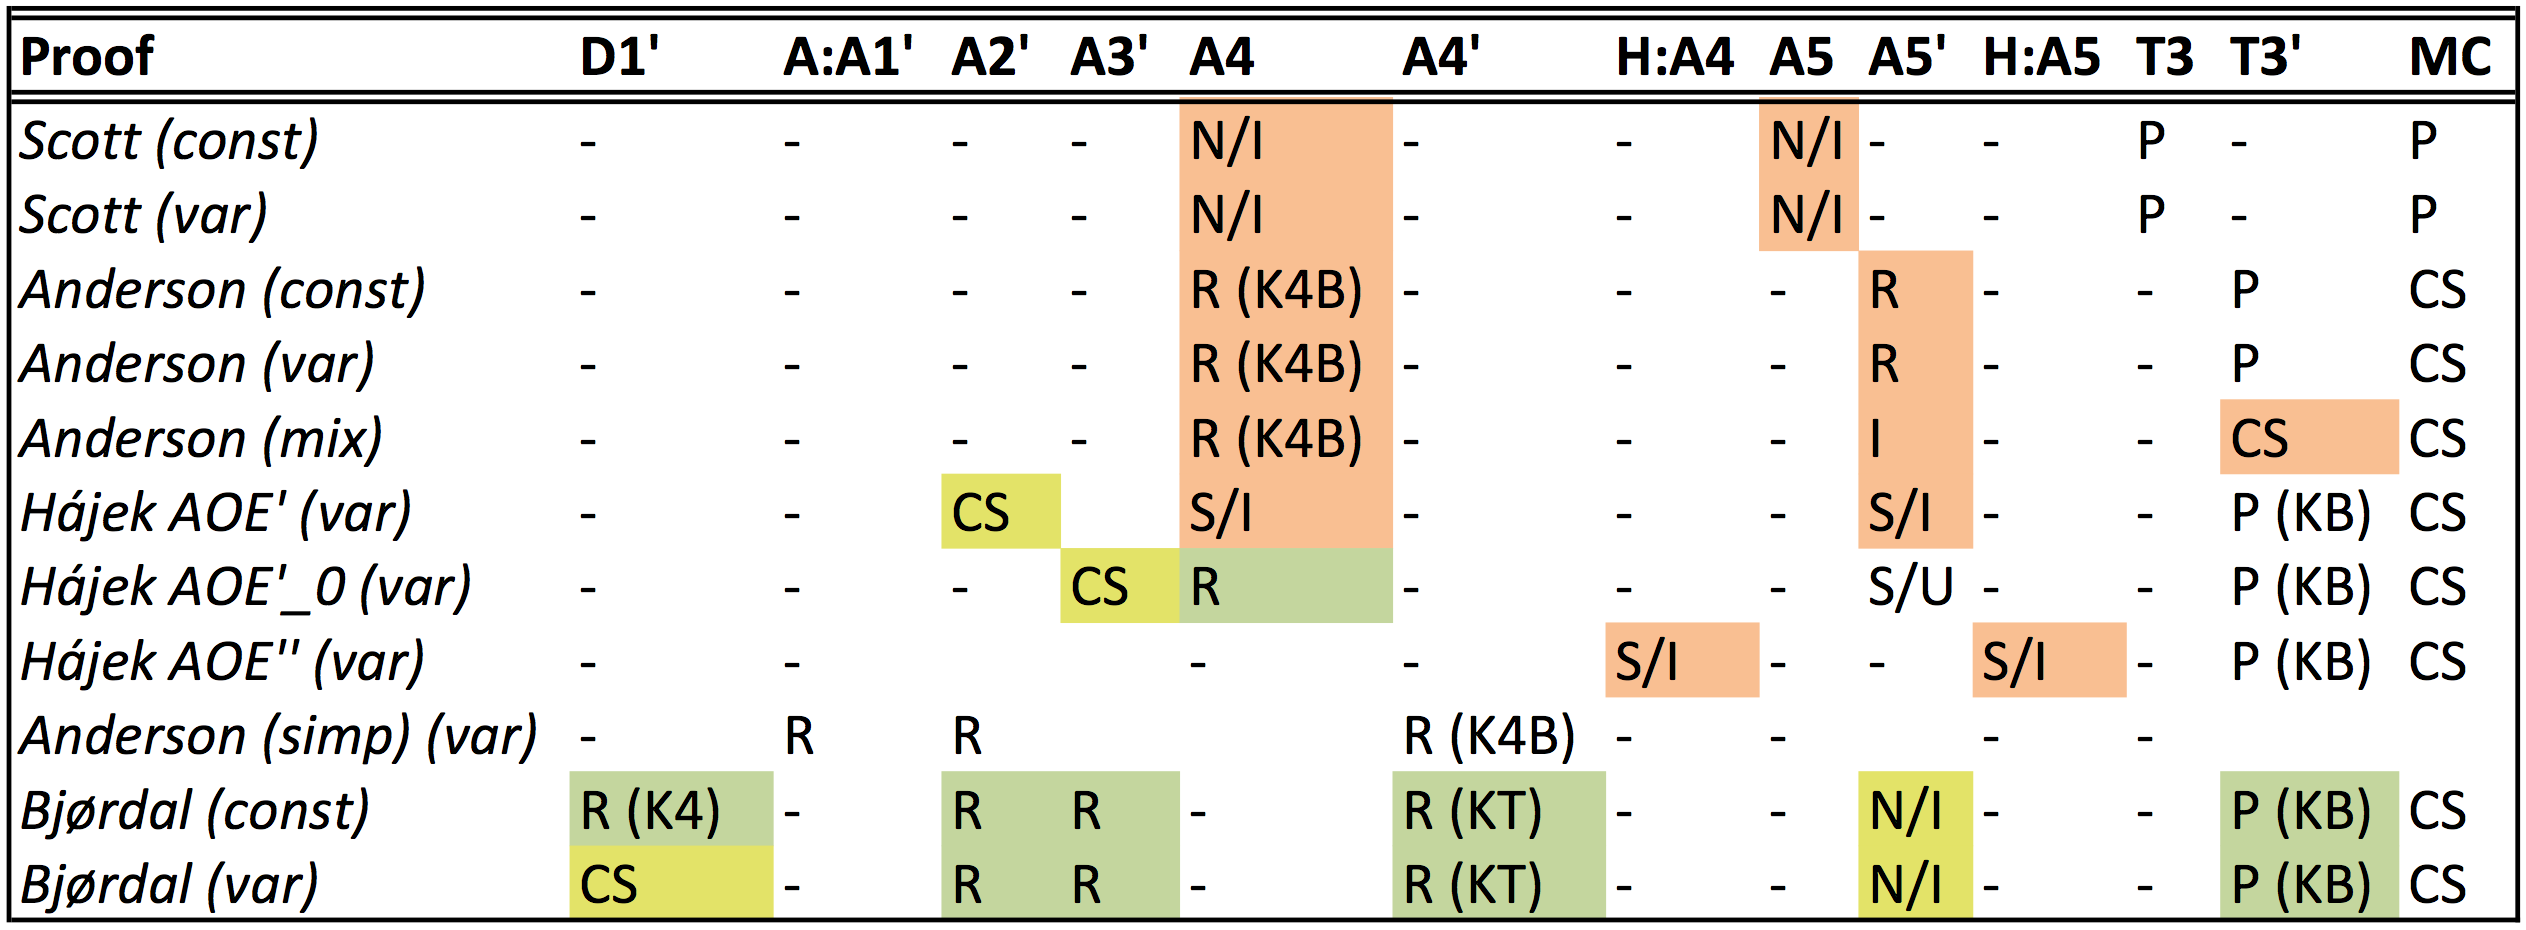
\includegraphics[width=1.2\textwidth]{Summary.png} 
\end{sideways}
%
\begin{sideways}
%\scalebox{.9}{
\resizebox{19cm}{4.5cm}{
\begin{tabular}{lccccccccccccc} 
\toprule
Investigated Variant & D1$'$ & A:A1$'$ & A2$'$ & A3$'$ & A4 & A4$'$ & H:A4 & A5 & A5$'$
  & H:A5 & T3 & T3$'$ & MC \\  
\midrule 
Scott (const) & - & - & - & - & \tabboxs{\tabred}{N/I} & - & - & \tabboxs{\tabred}{N/I} & - & - & P & -  & P \\
Scott (var) & - & - & - & - & \tabboxs{\tabred}{N/I} & - & - & \tabboxs{\tabred}{N/I} & - & - & P & -  & P \\
Anderson (const) & - & - & - & - & \tabbox{\tabred}{R(K4B)} & - & - & - & \tabboxs{\tabred}{R}  & - & - & P  & CS \\
Anderson (var) & - & - & - & - & \tabbox{\tabred}{R(K4B)} & - & - & - & \tabboxs{\tabred}{R}  & - & - & P  & CS \\
Anderson (mix) & - & - & - & - & \tabbox{\tabred}{R(K4B)} & - & - & - & \tabboxs{\tabred}{I}  & - & - & \tabboxs{\tabred}{CS} & CS \\
H\'ajek AOE$'$ (var) & - & - & \tabboxs{\tabyellow}{CS}  &  & \tabboxs{\tabred}{S/I} & - & - & - & \tabboxs{\tabred}{S/I}  & - & - & P(KB) & CS \\
H\'ajek AOE$'$\_0 (var) & - & - & - & \tabboxs{\tabyellow}{CS} & \tabboxs{\tabgreen}{R} & - & - & - & S/U & - & - & P(KB) & CS \\
H\'ajek AOE$''$ (var) & - & - &  &  & - & - & \tabboxs{\tabred}{S/I} & - & - & \tabboxs{\tabred}{S/I} & - & P(KB) & CS \\
Anderson (simp) (var) & - & R & R  &  &  & R(K4B) & - & - & & - & - &  & \\
Bjørdal (const) & \tabbox{\tabgreen}{R(K4)} & - & \tabboxs{\tabgreen}{R} & \tabboxs{\tabgreen}{R} & - & \tabbox{\tabgreen}{R(KT)} & - & - &\tabboxs{\tabyellow}{N/I} & - & - & \tabbox{\tabgreen}{P(KB)} &  CS \\
Bjørdal (var) & \tabboxs{\tabyellow}{CS} & - & \tabboxs{\tabgreen}{R} & \tabboxs{\tabgreen}{R} & - & \tabbox{\tabgreen}{R(KT)} & - & - &\tabboxs{\tabyellow}{N/I} & - & - & \tabbox{\tabgreen}{P(KB)} &  CS \\
\bottomrule
\end{tabular}
}
\end{sideways}
\caption{Summary of Results.}
\label{fig:summary}
\end{figure}

Figure \ref{fig:summary} summarizes the results obtained by the
automated reasoning tools. The following abbreviations are used: S/I =
superfluous and independent; R = superfluous and redundant; S/U =
superfluous and unknown whether redundant or independent; N/I =
non-superfluous and independent; P = provable; CS =
counter-satisfiable. The weakest logic required to show redundancy or
provability is indicated in parentheses (\K is the default).  Cells
highlighted in \colorbox{\tabred}{red} contain results that differ
from what had been claimed by either Magari, Anderson or Hájek. Cells
highlighted in \colorbox{\tabyellow}{yellow} contain results that are
surprising, albeit not contradicting any claims. Cells highlighted in
\colorbox{\tabgreen}{green} contain results where the tools were able
to obtain the same results as humans, but using weaker modal logics.
\footnote{EDNOTE: What is the difference between - and empty cells?}


\section{Conclusion}
Using our approach, that is, semantical embeddings of variants of higher-order
modal logics in classical higher-order logic, the formalization and
(partly) automated analysis of several variants of G\"odel's
ontological argument has been surprisingly straightforward. The
higher-order provers we employed not only confirmed many claimed results, but also exposed a
few mistakes and novel insights in a long standing controversy.  We
believe the technology employed in this work is ready to be fruitfully
adopted in larger scale by philosophers.  Moreover, our approach is
by no means restricted to metaphysics or philosophy, and further work
includes similar applications in other areas, including, for example,
law, politics and ethics. In fact, we claim, that our approach, at
least to some degree, realizes Leibniz' dream of a characteristica universalis
and calculus ratiocinator.



% ToDo: \\

% - Investigate Magari's proof

% - Hájek actually uses multi-sorted first-order formalizations. We should check that our results still hold in a multi-sorted first-order setting. They should.

% - Add apendix for Anderson's simplification

\sloppy
\printbibliography



% ------------------------------------------------------------------------
\end{document}
% ------------------------------------------------------------------------
